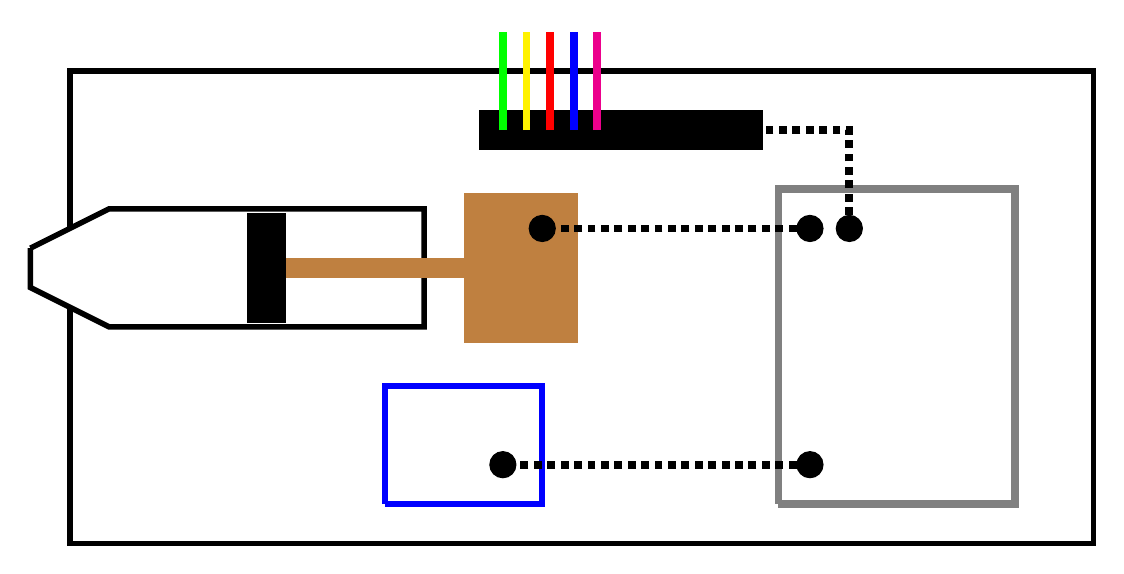
\begin{tikzpicture}
	% Hülle
	\draw[
		line width=0.07cm
	] (1,5) -- (1,2) -- (14,2) -- (14,8) -- (1,8) -- (1,6);
	% Spritze(oben)
	\draw[
		line width=0.07cm
	] (0.5,5.75) -- (0.5,5.25) -- (1.5,4.75) -- (5.5,4.75) -- (5.5,6.25) --
		(1.5,6.25) -- (0.5,5.75);
	% Arduino
	\draw[
		line width=0.1cm,
		color=gray
	] (10,2.5) -- (13,2.5) -- (13,6.5) -- (10,6.5) -- (10,2.5);
	% bluetooth
	\draw[
		line width=0.07cm,
		color=blue
	] (5,2.5) -- (5,4) -- (7,4) -- (7,2.5) -- (5,2.5);
	\node[
		circle,
		draw,
		fill=black
	] at (10.4,3) {};
	\node[
		circle,
		draw,
		fill=black
	] at (6.5,3) {};
	\draw[
		dotted,
		color=black,
		line width=0.1cm
	] (10.4,3) -- (6.5,3);
	% Servo(oben)
	\draw[
		line width=0.9cm,
		color=brown,
		fill=brown
	] (6,5) -- (7,5) -- (7,6) -- (6,6);
	% Kolben(oben)
	\draw[
		line width=0.5cm,
		color=black
	] (3.5,4.8) -- (3.5,6.2);
	% Verbindung Servo Kolben (oben)
	\draw[
		line width=0.25cm,
		color=brown
	] (3.75,5.5) -- (6,5.5);
	% Ansteuerung Servo (oben)
	\node[
		circle,
		draw,
		fill=black
	] at (10.4,6) {};
	\node[
		circle,
		draw,
		fill=black
	] at (7,6) {};
	\draw[
		dotted,
		color=black,
		line width=0.1cm
	] (10.4,6) -- (7,6);
	% Sensoren-Bank
	\draw[
		fill=black
	] (6.2,7) -- (9.8,7) -- (9.8,7.5) -- (6.2,7.5);
	% Sensoren
	\draw[
		color=green,
		line width=0.1cm
	] (6.5,7.25) -- (6.5,8.5);
	\draw[
		color=yellow,
		line width=0.1cm
	] (6.8,7.25) -- (6.8,8.5);
	\draw[
		color=red,
		line width=0.1cm
	] (7.1,7.25) -- (7.1,8.5);
	\draw[
		color=blue,
		line width=0.1cm
	] (7.4,7.25) -- (7.4,8.5);
	\draw[
		color=magenta,
		line width=0.1cm
	] (7.7,7.25) -- (7.7,8.5);
	% Sensoren Ansteuerung
	\node[
		circle,
		fill=black,
		draw
	] at (10.9,6) {};
	\draw[
		dotted,
		color=black,
		line width=0.1cm
	] (10.9,6) -- (10.9,7.25) -- (9.7,7.25);

\end{tikzpicture}
